\documentclass[aspectratio=169]{beamer}

% Theme and Color Setup
\usetheme{Madrid}
\usecolortheme{beaver}
\setbeamercolor{structure}{fg=darkred}

% Packages
\usepackage{tikz}
\usepackage{pgfplots}
\usepackage{amsmath}
\usepackage{booktabs}
\usepackage{caption}
\pgfplotsset{compat=1.17}
\usetikzlibrary{intersections, calc}

% Title Information
\title{Unit 3: Production, Cost, and Profit}
\subtitle{Based on Chapter 6: Costs of Production}
\author{Doğukan Günkördü}
\date{}

\begin{document}

% -----------------------------------------------------------------------------
% Title Slide
% -----------------------------------------------------------------------------
\begin{frame}
    \titlepage
\end{frame}

% -----------------------------------------------------------------------------
% Table of Contents
% -----------------------------------------------------------------------------
\begin{frame}{Outline}
    \tableofcontents
\end{frame}

% =============================================================================
% SECTION 1: The Production Function (Short Run vs Long Run)
% =============================================================================
\section{The Production Function}

\begin{frame}{Short Run vs. Long Run}
    \begin{block}{Defining the Time Periods}
        In economics, the difference between short and long run is not about days or years, but about \textbf{flexibility of resources}.
    \end{block}
    
    \vspace{0.5cm}
    
    \begin{columns}
        \column{0.5\textwidth}
        \textbf{The Short Run}
        \begin{itemize}
            \item At least \textbf{one} production input is \textbf{fixed} (usually capital/land).
            \item Supply cannot fully adjust to changes in demand.
            \item \textit{Example:} A farmer cannot buy more land immediately, but can hire more workers.
        \end{itemize}
        
        \column{0.5\textwidth}
        \textbf{The Long Run}
        \begin{itemize}
            \item \textbf{All} resources are \textbf{variable}.
            \item Firms can expand plant size or leave the industry.
            \item Supply can fully adjust.
        \end{itemize}
    \end{columns}
\end{frame}

\begin{frame}{Key Production Terms}
    To understand costs, we first look at production (inputs $\rightarrow$ outputs).
    
    \begin{itemize}
        \item \textbf{Total Product (TP):} The total quantity of output produced.
        \item \textbf{Marginal Product (MP):} The additional output produced by adding one more unit of input (labor).
        \[ MP = \frac{\Delta \text{Total Product}}{\Delta \text{Inputs}} \]
        \item \textbf{Average Product (AP):} The output per unit of input.
        \[ AP = \frac{\text{Total Product}}{\text{Units of Labor}} \]
    \end{itemize}
\end{frame}

\begin{frame}{Law of Diminishing Marginal Returns}
    \begin{alertblock}{The Law}
        As variable inputs (labor) are added to a \textbf{fixed} resource (capital), the additional output produced by each new worker will eventually fall.
    \end{alertblock}

    \textbf{Three Stages of Returns:}
    \begin{enumerate}
        \item \textbf{Increasing Marginal Returns:} Specialization allows MP to rise. TP increases at an increasing rate.
        \item \textbf{Diminishing Marginal Returns:} Fixed resources get overcrowded. MP is positive but falling. TP increases at a decreasing rate.
        \item \textbf{Negative Marginal Returns:} Workers get in each other's way. MP is negative. TP falls.
    \end{enumerate}
\end{frame}

\begin{frame}{Graphing Production Functions}
    \begin{columns}
        \column{0.4\textwidth}
        \textbf{Key Relationships:}
        \begin{itemize}
            \item MP intersects AP at AP's maximum.
            \item If $MP > AP$, AP is rising.
            \item If $MP < AP$, AP is falling.
            \item TP is maximized when $MP = 0$.
        \end{itemize}
        
        \column{0.6\textwidth}
        \centering
        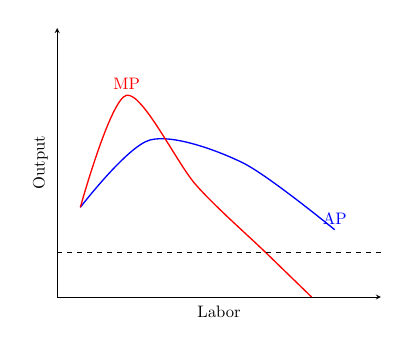
\begin{tikzpicture}[scale=0.6]
            \begin{axis}[
                axis lines=left,
                xlabel={Labor},
                ylabel={Output},
                ymin=-2, ymax=10,
                xmin=0, xmax=7,
                xtick=\empty, ytick=\empty,
                clip=false,
            ]
                % AP Curve
                \addplot[blue, thick, smooth] coordinates {(0.5,2) (2,5) (4,4) (6,1)};
                \node[blue] at (axis cs: 6,1.5) {AP};
                
                % MP Curve
                \addplot[red, thick, smooth] coordinates {(0.5,2) (1.5,7) (3,3) (4.5,0) (5.5,-2)};
                \node[red] at (axis cs: 1.5,7.5) {MP};
                
                \draw[dashed] (axis cs:0,0) -- (axis cs:7,0);
            \end{axis}
        \end{tikzpicture}
    \end{columns}
\end{frame}

% =============================================================================
% SECTION 2: Short-Run Costs
% =============================================================================
\section{Short-Run Costs}

\begin{frame}{Classifying Costs}
    \begin{columns}
        \column{0.5\textwidth}
        \textbf{1. Fixed Costs (FC)}
        \begin{itemize}
            \item Do \textbf{not} vary with output.
            \item Must be paid even if Output = 0.
            \item \textit{Examples:} Rent, insurance, machinery.
        \end{itemize}
        
        \column{0.5\textwidth}
        \textbf{2. Variable Costs (VC)}
        \begin{itemize}
            \item Change as output changes.
            \item If Output = 0, VC = 0.
            \item \textit{Examples:} Wages, raw materials, electricity.
        \end{itemize}
    \end{columns}
    
    \vspace{0.5cm}
    \begin{center}
        \Large \textbf{Total Cost (TC) = TFC + TVC}
    \end{center}
\end{frame}

\begin{frame}{Per-Unit Cost Formulas}
    You must memorize these formulas. They are the average of the totals.
    
    \begin{table}
        \centering
        \renewcommand{\arraystretch}{1.5}
        \begin{tabular}{l c l}
            \toprule
            \textbf{Measure} & \textbf{Formula} & \textbf{Shape} \\
            \midrule
            Average Fixed Cost (AFC) & $\frac{\text{TFC}}{Q}$ & Always declines as Q rises \\
            Average Variable Cost (AVC) & $\frac{\text{TVC}}{Q}$ & U-shaped \\
            Average Total Cost (ATC) & $\frac{\text{TC}}{Q} \text{ or } AFC + AVC$ & U-shaped \\
            \textbf{Marginal Cost (MC)} & $\frac{\Delta \text{TC}}{\Delta Q}$ & Nike Swoosh ($\checkmark$) \\
            \bottomrule
        \end{tabular}
    \end{table}
\end{frame}

\begin{frame}{The Marginal Cost Curve (MC)}
    \begin{columns}
        \column{0.6\textwidth}
        \textbf{Why is MC so important?}
        \begin{itemize}
            \item MC is the cost of producing the \textit{next} unit.
            \item \textbf{Mirror Image:} MC is the mirror image of Marginal Product.
            \item When MP is rising (specialization), MC is falling.
            \item When Diminishing Returns set in (MP falls), MC begins to rise.
        \end{itemize}
        
        \column{0.4\textwidth}
        \begin{block}{Geometry Tip}
            The MC curve looks like a Nike swoosh. It always cuts through the \textbf{minimum} points of the ATC and AVC curves.
        \end{block}
    \end{columns}
\end{frame}

\begin{frame}{Visualizing Short-Run Cost Curves}
    \centering
    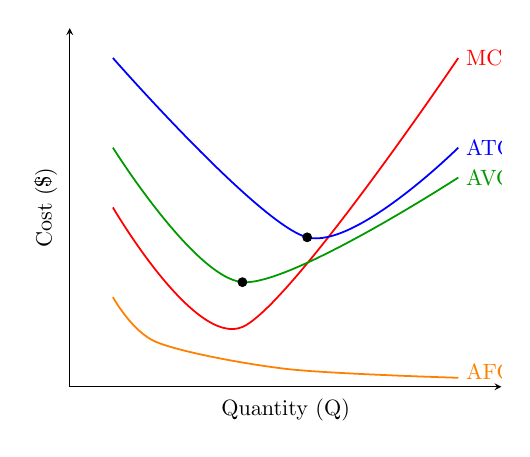
\begin{tikzpicture}[scale=0.8]
        \begin{axis}[
            axis lines=left,
            xlabel={Quantity (Q)},
            ylabel={Cost (\$)},
            ymin=0, ymax=12,
            xmin=0, xmax=10,
            xtick=\empty, ytick=\empty,
        ]
            % MC Curve (Swoosh)
            \addplot[red, thick, smooth] coordinates {(1,6) (4,2) (9,11)};
            \node[red, right] at (axis cs:9,11) {MC};

            % ATC Curve (U-shape, above AVC)
            \addplot[blue, thick, smooth] coordinates {(1,11) (5.5,5) (9,8)};
            \node[blue, right] at (axis cs:9,8) {ATC};

            % AVC Curve (U-shape, below ATC, gets closer)
            \addplot[green!60!black, thick, smooth] coordinates {(1,8) (4,3.5) (9,7)};
            \node[green!60!black, right] at (axis cs:9,7) {AVC};

            % AFC Curve (Falling asymptote)
            \addplot[orange, thick, smooth] coordinates {(1,3) (2,1.5) (5,0.6) (9,0.3)};
            \node[orange, right] at (axis cs:9,0.5) {AFC};
            
            % Intersection Dots
            \filldraw[black] (axis cs:5.5,5) circle (2pt); % Min ATC
            \filldraw[black] (axis cs:4,3.5) circle (2pt); % Min AVC
            
        \end{axis}
    \end{tikzpicture}
    
    \small Note: Vertical distance between ATC and AVC represents AFC.
\end{frame}

% =============================================================================
% SECTION 3: Shifting Cost Curves (Taxes)
% =============================================================================
\section{Shifting Cost Curves}

\begin{frame}{Impact of Taxes on Costs}
    How do taxes shift the curves? It depends on the type of tax.
    
    \vspace{0.5cm}
    
    \begin{columns}
        \column{0.5\textwidth}
        \begin{block}{1. Per-Unit Tax}
            \begin{itemize}
                \item Tax on every unit produced (e.g., excise tax).
                \item Acts like a \textbf{Variable Cost}.
                \item \textbf{Shifts:} MC, AVC, and ATC shift \textbf{UP}.
                \item \textbf{Result:} Changes profit-maximizing quantity ($MR=MC$).
            \end{itemize}
        \end{block}
        
        \column{0.5\textwidth}
        \begin{block}{2. Lump-Sum Tax}
            \begin{itemize}
                \item One-time fixed tax regardless of output (e.g., license fee).
                \item Acts like a \textbf{Fixed Cost}.
                \item \textbf{Shifts:} Only AFC and ATC shift \textbf{UP}.
                \item \textbf{Result:} MC does \textbf{not} change, so quantity produced stays the same.
            \end{itemize}
        \end{block}
    \end{columns}
\end{frame}

% =============================================================================
% SECTION 4: Long-Run Costs
% =============================================================================
\section{Long-Run Costs}

\begin{frame}{Long-Run Average Total Cost (LRATC)}
    In the long run, firms can change plant size. The LRATC curve acts as an "envelope" curve containing all possible short-run ATC curves.
    
    \vspace{0.3cm}
    \textbf{Three Phases of LRATC:}
    \begin{enumerate}
        \item \textbf{Economies of Scale:} Long-run average cost \textit{falls} as output increases. (Mass production efficiency).
        \item \textbf{Constant Returns to Scale:} Long-run average cost stays the same as output increases.
        \item \textbf{Diseconomies of Scale:} Long-run average cost \textit{rises} as output increases. (Firm gets too big to manage efficiently).
    \end{enumerate}
\end{frame}

\begin{frame}{Visualizing Economies of Scale}
    \centering
    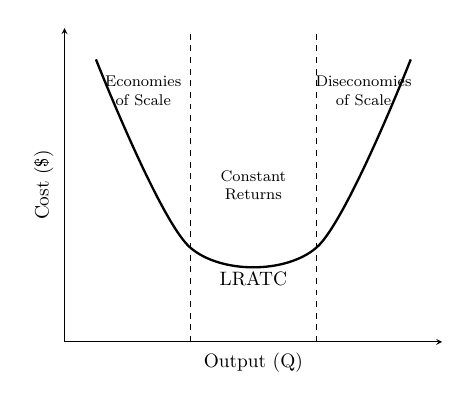
\begin{tikzpicture}[scale=0.7]
        \begin{axis}[
            axis lines=left,
            xlabel={Output (Q)},
            ylabel={Cost (\$)},
            ymin=0, ymax=10,
            xmin=0, xmax=12,
            xtick=\empty, ytick=\empty,
        ]
            % LRATC - Saucer Shape
            \addplot[black, very thick, smooth] coordinates {(1,9) (4,3) (8,3) (11,9)};
            \node at (axis cs:6, 2) {LRATC};
            
            % Zones
            \draw[dashed] (axis cs:4,0) -- (axis cs:4,10);
            \draw[dashed] (axis cs:8,0) -- (axis cs:8,10);
            
            \node[align=center, font=\footnotesize] at (axis cs:2.5, 8) {Economies\\of Scale};
            \node[align=center, font=\footnotesize] at (axis cs:6, 5) {Constant\\Returns};
            \node[align=center, font=\footnotesize] at (axis cs:9.5, 8) {Diseconomies\\of Scale};
        \end{axis}
    \end{tikzpicture}
\end{frame}

% =============================================================================
% SECTION 5: Profit Definitions
% =============================================================================
\section{Economic vs. Accounting Profit}

\begin{frame}{Types of Profit}
    \begin{columns}
        \column{0.5\textwidth}
        \textbf{Accountants}
        \begin{itemize}
            \item Look only at \textbf{Explicit Costs} (out-of-pocket payments like wages, rent).
            \item $ \text{Acct Profit} = \text{TR} - \text{Explicit Costs} $
        \end{itemize}
        
        \column{0.5\textwidth}
        \textbf{Economists}
        \begin{itemize}
            \item Look at Explicit \textbf{AND Implicit Costs}.
            \item \textbf{Implicit Cost:} Opportunity cost (forgone income).
            \item $ \text{Econ Profit} = \text{TR} - (\text{Explicit} + \text{Implicit}) $
        \end{itemize}
    \end{columns}
    
    \vspace{0.5cm}
    \begin{alertblock}{Normal Profit}
        When \textbf{Economic Profit = 0}. This means the firm is breaking even by economic standards and resources are being used efficiently. The owner is making exactly what they would in their next best alternative.
    \end{alertblock}
\end{frame}

\begin{frame}{Example: Bron's Burrito Shop}
    LeBron James retires to open a burrito shop.
    \begin{itemize}
        \item \textbf{Revenue:} \$3 Million
        \item \textbf{Explicit Costs} (Rent, wages, food): \$2 Million
        \item \textbf{Implicit Costs} (Lost NBA Salary): \$20 Million
    \end{itemize}
    
    \vspace{0.5cm}
    
    \begin{columns}
        \column{0.5\textwidth}
        \textbf{Accounting Profit:}
        \[ \$3M - \$2M = \textbf{+\$1 Million} \]
        \textit{"Great year!"}
        
        \column{0.5\textwidth}
        \textbf{Economic Profit:}
        \[ \$3M - (\$2M + \$20M) = \textbf{-\$19 Million} \]
        \textit{"Terrible decision!"}
    \end{columns}
\end{frame}

\begin{frame}{Summary Checklist for Unit 3}
    \begin{itemize}
        \item[$\square$] Differentiate Fixed vs. Variable resources (Short vs Long run).
        \item[$\square$] Calculate MP and identify Diminishing Marginal Returns.
        \item[$\square$] Draw and label MC, ATC, AVC, AFC.
        \item[$\square$] Ensure MC cuts ATC and AVC at minimum points.
        \item[$\square$] Shift curves correctly for Per-Unit vs. Lump-Sum taxes.
        \item[$\square$] Calculate Economic Profit vs. Accounting Profit.
    \end{itemize}
\end{frame}

\end{document}
